% GNUPLOT: LaTeX picture with Postscript
\begingroup
  \makeatletter
  \providecommand\color[2][]{%
    \GenericError{(gnuplot) \space\space\space\@spaces}{%
      Package color not loaded in conjunction with
      terminal option `colourtext'%
    }{See the gnuplot documentation for explanation.%
    }{Either use 'blacktext' in gnuplot or load the package
      color.sty in LaTeX.}%
    \renewcommand\color[2][]{}%
  }%
  \providecommand\includegraphics[2][]{%
    \GenericError{(gnuplot) \space\space\space\@spaces}{%
      Package graphicx or graphics not loaded%
    }{See the gnuplot documentation for explanation.%
    }{The gnuplot epslatex terminal needs graphicx.sty or graphics.sty.}%
    \renewcommand\includegraphics[2][]{}%
  }%
  \providecommand\rotatebox[2]{#2}%
  \@ifundefined{ifGPcolor}{%
    \newif\ifGPcolor
    \GPcolorfalse
  }{}%
  \@ifundefined{ifGPblacktext}{%
    \newif\ifGPblacktext
    \GPblacktexttrue
  }{}%
  % define a \g@addto@macro without @ in the name:
  \let\gplgaddtomacro\g@addto@macro
  % define empty templates for all commands taking text:
  \gdef\gplbacktext{}%
  \gdef\gplfronttext{}%
  \makeatother
  \ifGPblacktext
    % no textcolor at all
    \def\colorrgb#1{}%
    \def\colorgray#1{}%
  \else
    % gray or color?
    \ifGPcolor
      \def\colorrgb#1{\color[rgb]{#1}}%
      \def\colorgray#1{\color[gray]{#1}}%
      \expandafter\def\csname LTw\endcsname{\color{white}}%
      \expandafter\def\csname LTb\endcsname{\color{black}}%
      \expandafter\def\csname LTa\endcsname{\color{black}}%
      \expandafter\def\csname LT0\endcsname{\color[rgb]{1,0,0}}%
      \expandafter\def\csname LT1\endcsname{\color[rgb]{0,1,0}}%
      \expandafter\def\csname LT2\endcsname{\color[rgb]{0,0,1}}%
      \expandafter\def\csname LT3\endcsname{\color[rgb]{1,0,1}}%
      \expandafter\def\csname LT4\endcsname{\color[rgb]{0,1,1}}%
      \expandafter\def\csname LT5\endcsname{\color[rgb]{1,1,0}}%
      \expandafter\def\csname LT6\endcsname{\color[rgb]{0,0,0}}%
      \expandafter\def\csname LT7\endcsname{\color[rgb]{1,0.3,0}}%
      \expandafter\def\csname LT8\endcsname{\color[rgb]{0.5,0.5,0.5}}%
    \else
      % gray
      \def\colorrgb#1{\color{black}}%
      \def\colorgray#1{\color[gray]{#1}}%
      \expandafter\def\csname LTw\endcsname{\color{white}}%
      \expandafter\def\csname LTb\endcsname{\color{black}}%
      \expandafter\def\csname LTa\endcsname{\color{black}}%
      \expandafter\def\csname LT0\endcsname{\color{black}}%
      \expandafter\def\csname LT1\endcsname{\color{black}}%
      \expandafter\def\csname LT2\endcsname{\color{black}}%
      \expandafter\def\csname LT3\endcsname{\color{black}}%
      \expandafter\def\csname LT4\endcsname{\color{black}}%
      \expandafter\def\csname LT5\endcsname{\color{black}}%
      \expandafter\def\csname LT6\endcsname{\color{black}}%
      \expandafter\def\csname LT7\endcsname{\color{black}}%
      \expandafter\def\csname LT8\endcsname{\color{black}}%
    \fi
  \fi
    \setlength{\unitlength}{0.0500bp}%
    \ifx\gptboxheight\undefined%
      \newlength{\gptboxheight}%
      \newlength{\gptboxwidth}%
      \newsavebox{\gptboxtext}%
    \fi%
    \setlength{\fboxrule}{0.5pt}%
    \setlength{\fboxsep}{1pt}%
\begin{picture}(5400.00,3780.00)%
    \gplgaddtomacro\gplbacktext{%
      \csname LTb\endcsname%%
      \put(1078,704){\makebox(0,0)[r]{\strut{}2.710}}%
      \csname LTb\endcsname%%
      \put(1078,989){\makebox(0,0)[r]{\strut{}2.715}}%
      \csname LTb\endcsname%%
      \put(1078,1275){\makebox(0,0)[r]{\strut{}2.720}}%
      \csname LTb\endcsname%%
      \put(1078,1560){\makebox(0,0)[r]{\strut{}2.725}}%
      \csname LTb\endcsname%%
      \put(1078,1846){\makebox(0,0)[r]{\strut{}2.730}}%
      \csname LTb\endcsname%%
      \put(1078,2131){\makebox(0,0)[r]{\strut{}2.735}}%
      \csname LTb\endcsname%%
      \put(1078,2417){\makebox(0,0)[r]{\strut{}2.740}}%
      \csname LTb\endcsname%%
      \put(1078,2702){\makebox(0,0)[r]{\strut{}2.745}}%
      \csname LTb\endcsname%%
      \put(1078,2988){\makebox(0,0)[r]{\strut{}2.750}}%
      \csname LTb\endcsname%%
      \put(1078,3273){\makebox(0,0)[r]{\strut{}2.755}}%
      \csname LTb\endcsname%%
      \put(1078,3559){\makebox(0,0)[r]{\strut{}2.760}}%
      \csname LTb\endcsname%%
      \put(1210,484){\makebox(0,0){\strut{}4}}%
      \csname LTb\endcsname%%
      \put(1752,484){\makebox(0,0){\strut{}8}}%
      \csname LTb\endcsname%%
      \put(2294,484){\makebox(0,0){\strut{}12}}%
      \csname LTb\endcsname%%
      \put(2836,484){\makebox(0,0){\strut{}16}}%
      \csname LTb\endcsname%%
      \put(3377,484){\makebox(0,0){\strut{}24}}%
      \csname LTb\endcsname%%
      \put(3919,484){\makebox(0,0){\strut{}32}}%
      \csname LTb\endcsname%%
      \put(4461,484){\makebox(0,0){\strut{}48}}%
      \csname LTb\endcsname%%
      \put(5003,484){\makebox(0,0){\strut{}64}}%
    }%
    \gplgaddtomacro\gplfronttext{%
      \csname LTb\endcsname%%
      \put(209,2131){\rotatebox{-270}{\makebox(0,0){\strut{}Energy (a.u.)}}}%
      \put(3106,154){\makebox(0,0){\strut{}Basis size (unitless)}}%
      \csname LTb\endcsname%%
      \put(3769,3164){\makebox(0,0)[r]{\strut{}$E_\mathrm{GP}$}}%
      \csname LTb\endcsname%%
      \put(3769,2944){\makebox(0,0)[r]{\strut{}$E_\mathrm{PT}$}}%
      \csname LTb\endcsname%%
      \put(3769,2724){\makebox(0,0)[r]{\strut{}$E_\mathrm{CI}$}}%
    }%
    \gplbacktext
    \put(0,0){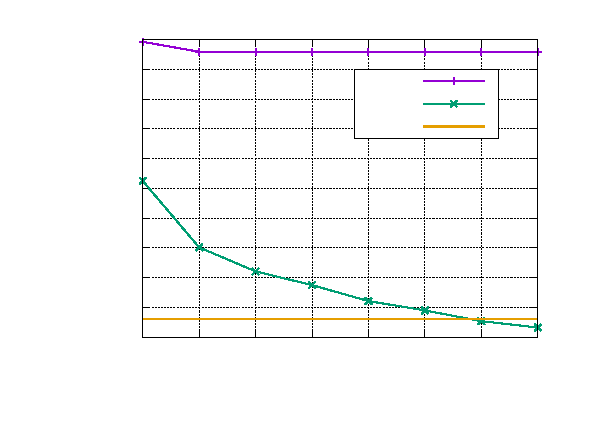
\includegraphics[width={270.00bp},height={189.00bp}]{imgs/gp_pt_cisd}}%
    \gplfronttext
  \end{picture}%
\endgroup
